\documentclass[8pt]{beamer}
    \usepackage{graphicx}
    \usepackage{wrapfig}
    \usepackage{multicol}

    \usepackage[T1]{fontenc}
    \usepackage{mathptmx}
    \usetheme{Madrid}
    
    \title{Building permits - Chi}
    \author{Ahmed Ayman}
    
    \begin{document}
        \maketitle
        \begin{frame}{Agenda}
            \begin{itemize}
                \item The story
                \item Dataset
                \item From Business to statistics
            \end{itemize}
        \end{frame}

        \begin{frame}{The story}
            A house inspector randomly samples building permits pulled by  69 little pigs who were building houses.\\
            \textbf{Wonder if there a preference for materials}\\
            materials categories: [brick, sticks, straw]\\
            \centering
            
\includegraphics[height=.33\textheight]{images/pig.jpg}
            \begin{columns}
                \column{.33\textwidth}
                \centering
                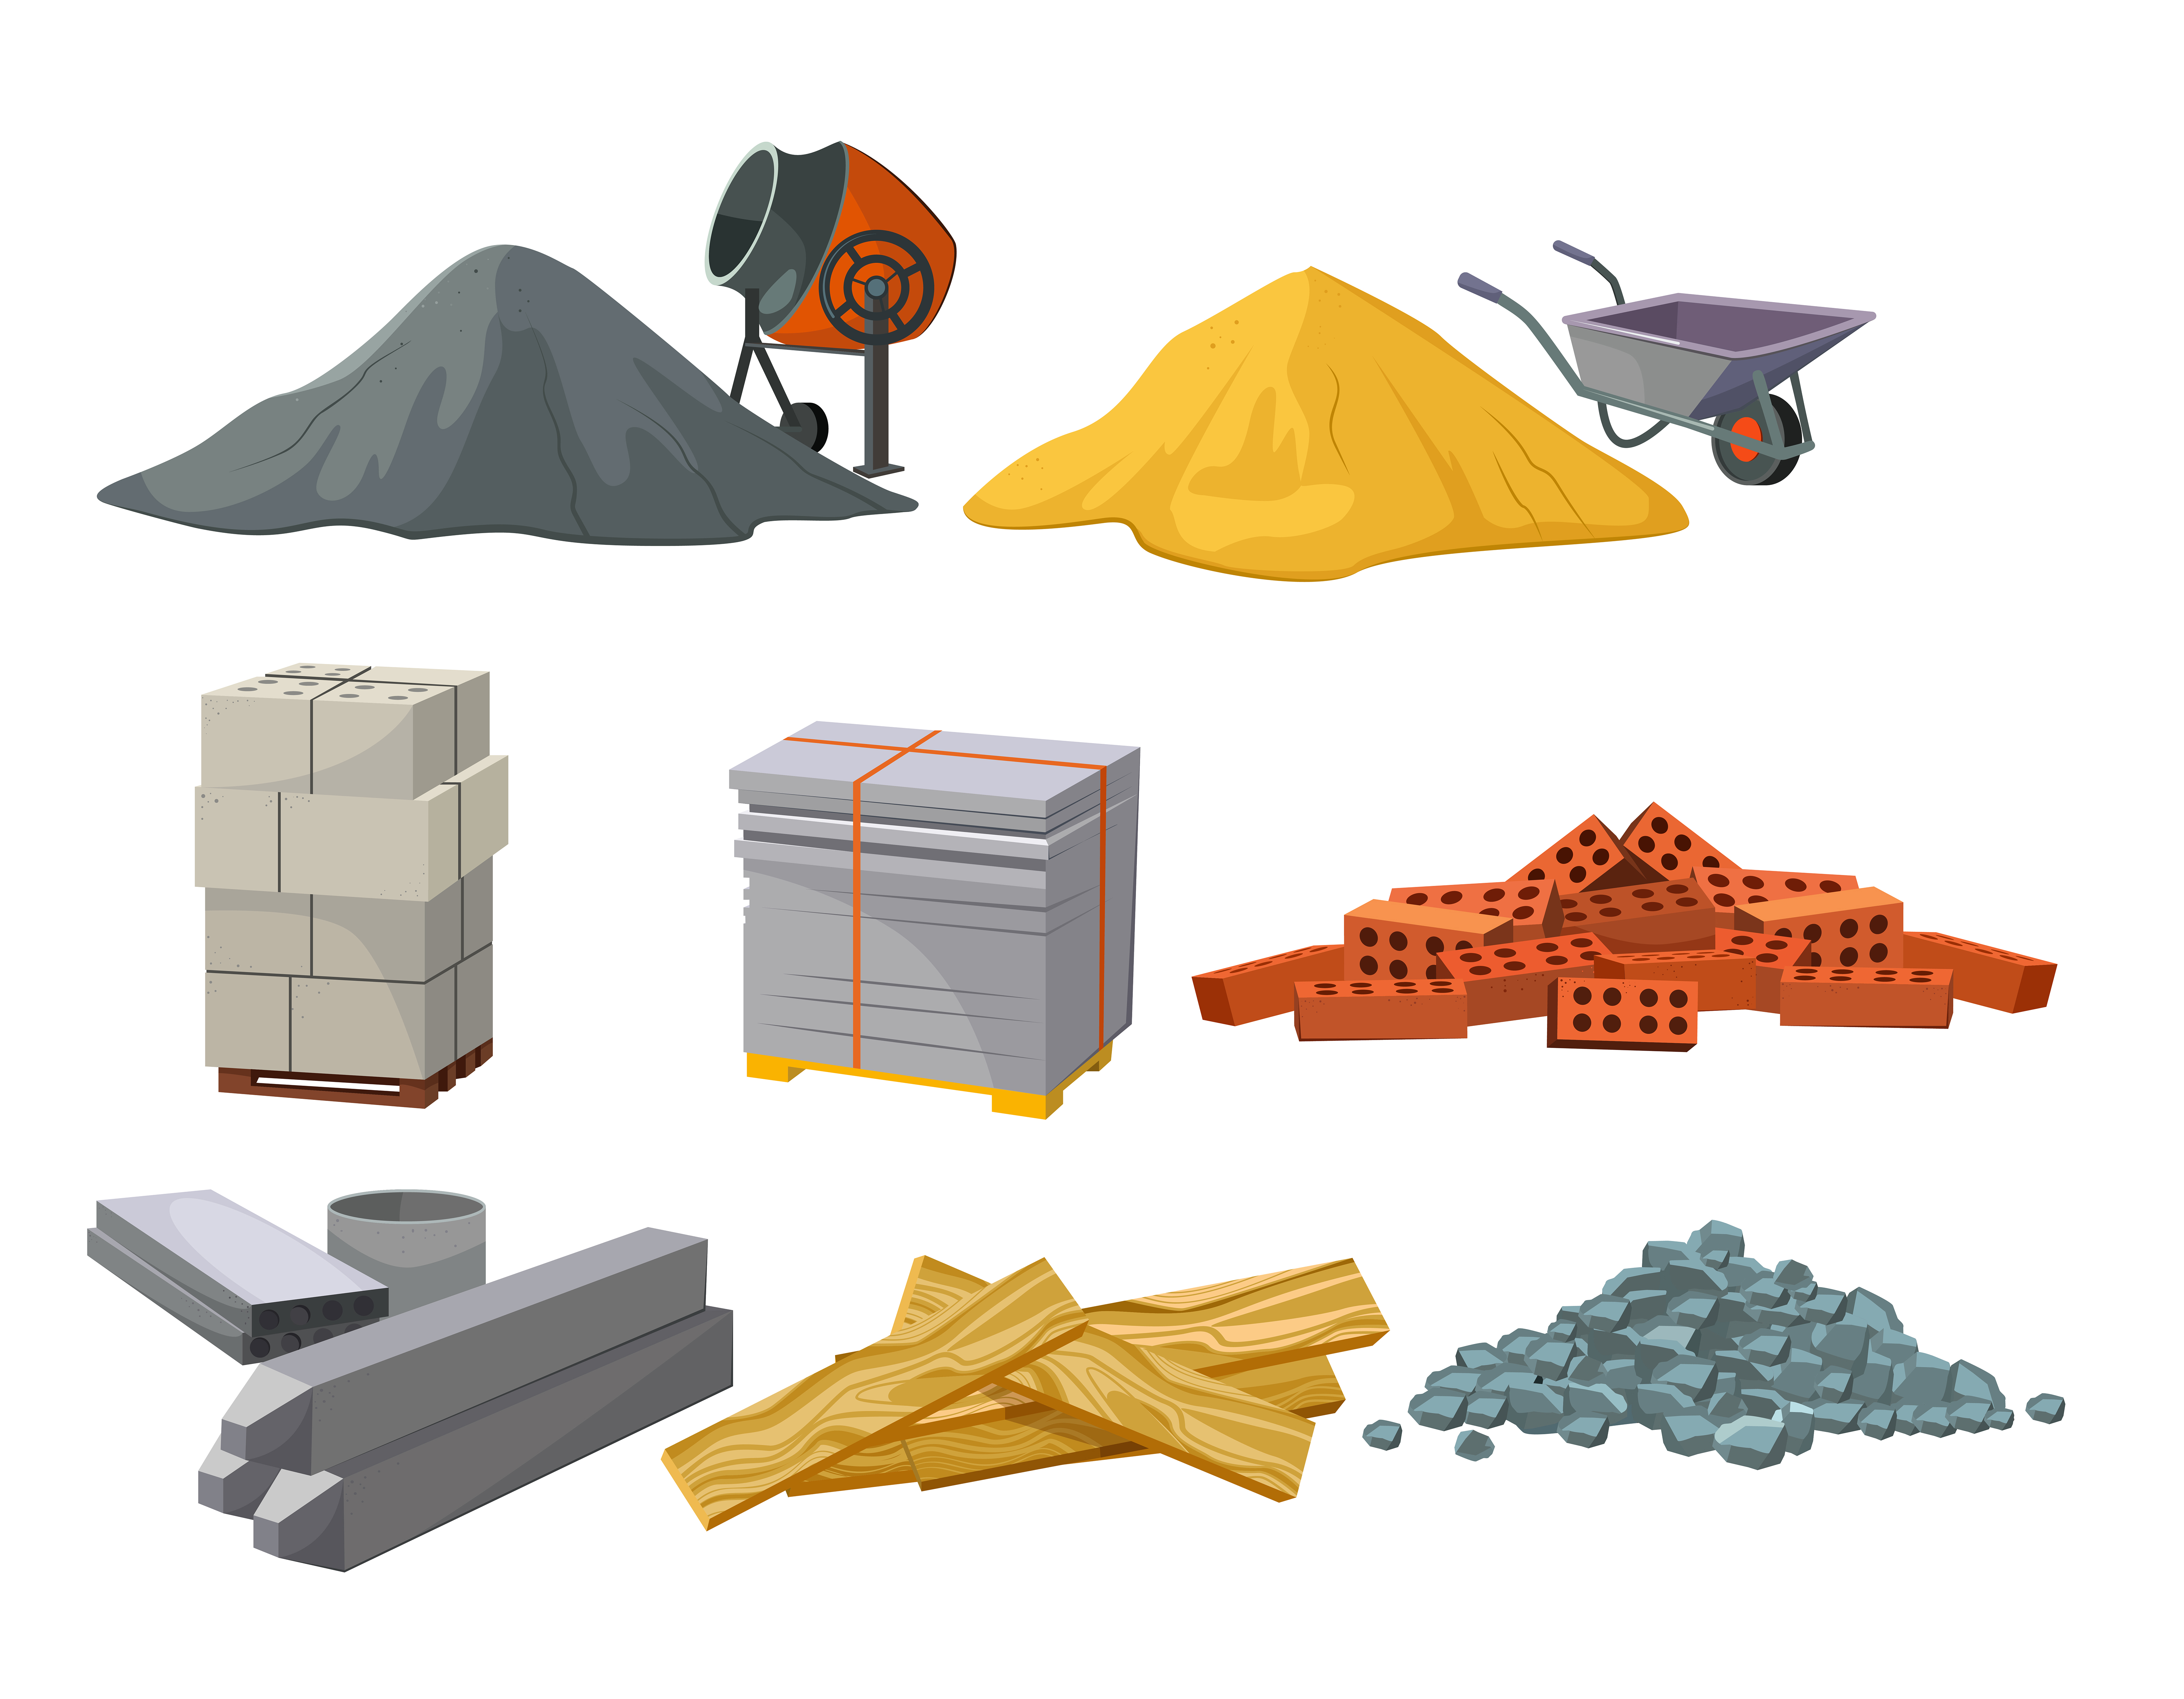
\includegraphics[width=.95\textwidth]{images/brick}
                \column{.33\textwidth}
                \centering
                
\includegraphics[width=.95\textwidth]{images/sticks}
                \column{.33\textwidth}
                \centering
                
\includegraphics[width=.95\textwidth]{images/straw}
            \end{columns}
        \end{frame}

        \begin{frame}[t]{Dataset}
            Our Data contains two columns
            \begin{itemize}
                \item \textbf{materials:} Name of the material
                \item \textbf{permits:} number of building found with the material
            \end{itemize}\\[1.5cm]
            \centering
            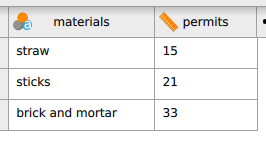
\includegraphics[height=.25\textheight]{images/data.png}
        \end{frame}

        \begin{frame}{From Business to statistics}
            \begin{block}{\textbf{Questions}}
                \begin{itemize}
                    \item \textbf{Business:} is there preference in material?!
                    \item \textbf{Statistical:} permits(material 1) = permits(material 2) \ldots = permits(material n)
                    \item The Statistical test is \textcolor{red}{\textbf{Chi-square}} (Hope: this test to be statistically significant)
                \end{itemize}
            \end{block}

            \begin{block}{\textbf{test result}}
                \begin{columns}
                    \column{.45\textwidth}
                    \begin{itemize}
                        \item The p-value is much less than .05
                        \item Which means there is preference
                        \item \item So, we confidently reject the $H_0$
                        \item \textcolor{blue}{\textbf{Great}}
                    \end{itemize}
                    \column{.55\textwidth}
                    \begin{figure}
                        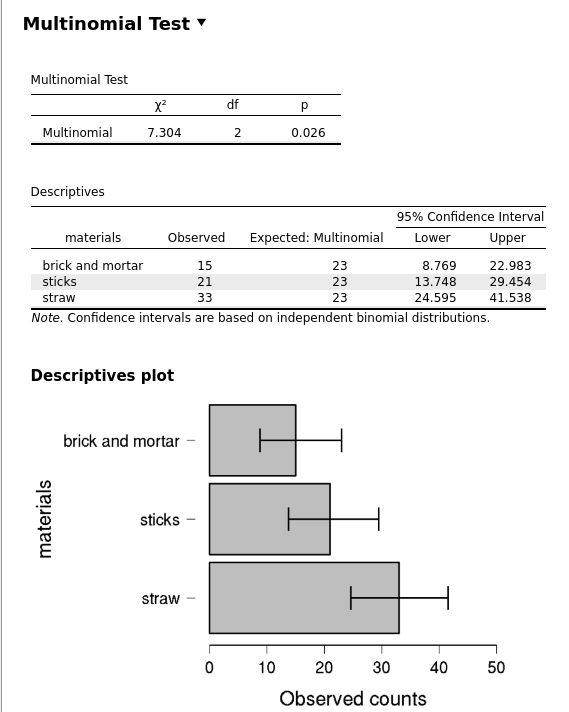
\includegraphics[height=.5\textheight]{images/chi.png}
                    \end{figure}
                \end{columns}
            \end{block}
        \end{frame}
    \end{document}